% !TEX root = ../main_lecture_notes.tex
\chapter{Mouvement brownien}\label{chap:mb}
Le contenu de ce chapitre s'inspire de l'ouvrage de \citet{Dobrow2016} et des notes de cours de \citet{MJB06}.
\section{Un peu d'histoire}
\begin{itemize}
  \item[1827] Le botaniste écossais Robert Brown (1773-1858) en immergeant dans un liquide au repos des grains de pollen de la Clarkia pulchella (une espèce de fleur sauvage nordaméricaine d’environ 100 microns) remarqua un comportement désordonné. Il observa au microscope de minuscules particules de quelques micromètres décrivant à la surface du liquide des trajectoires apparemment erratiques. Il utilisa les grains de pollen car ils contenaient des particules oblongues ayant une forme allongée plus longue que large. Brown était particulièrement passionné par les pollens et il croyait pouvoir suivre leur progression durant la fertilisation. Il pensait que ce mouvement était causé par un fluide vital provenant de l’intérieur des grains de pollen. En apprenant qu’Ingenkousz avait observé le même comportement pour la poussière de charbon, Brown renonça à son hypothèse du fluide vital et il réussit à montrer que ce mouvement chaotique se produisait également avec des grains de matière inerte.  En 1828, Brown publia ses résultats dans un article2 de la revue The Edinburgh Journal of Science.
  \item[1877] ELe physicien Joseph Delsaux (1828-1891) et le mathématicien Père Jésuite Ignace Carbonnelle (1829-1889) ont émis l’hypothèse selon laquelle les changements continus de direction de trajectoires qui donnent lieu au mouvement aléatoire et erratique des grains de pollen, sont dus aux chocs incessants entre les particules de pollen et les innombrables molécules d’eau qui sont comparativement beaucoup plus petites que les grains de pollen. Par conséquent, les petites particules contenues dans les grains de pollen de la Clarkia pulchella se déplaceraient de façon erratique, car elles seraient heurtées ou bombardées par des entités invisibles nommément, les molécules d’eau dans lesquelles elles sont immergées. Comme ces molécules sont soumises en permanence à une agitation thermique, les particules se déplacent nécessairement les unes par rapport aux autres. 
  \item[1900] Louis Bachelier soutien à la Sorbonne sa thèse de doctorat intitulée « Théorie de la spéculation » rédigée sous la direction du célèbre mathématicien Henri Poincaré. Dans cette thèse, Bachelier utilise l’idée du mouvement brownien pour modéliser la dynamique des prix des actions à la bourse de Paris. Sa thèse contenait, entre autres, cette idée de lier les fluctuations boursières à l’équation de la chaleur. Cette thèse fut le début de la finance moderne et le point de départ de la théorie des produits dérivés qui s’appelaient à l’époque produits à prime. De nos jours, le mouvement brownien est omniprésent dans le modèle de Black-Scholes pour calculer la valeur théorique de certains contrats d’option, en utilisant les cours boursiers actuels, les dividendes attendus, le prix d’exercice de l’option, les taux d’intérêt, le délai d’expiration et la volatilité.
  \item[1905] Albert Einstein a donné une description quantitative du mouvement brownien et a modélisé pour la première fois le mouvement des particules dans un liquide soumises à des interactions aléatoires. Son article5 de 1905 étudie la probabilité qu’une particule se trouve en un endroit donné en un instant t. Cet article marque la naissance de la physique statistique.
  \begin{enumerate}
    \item Le mouvement de chaque particule est indépendant des mouvements des autres particules.
    \item Les mouvements d’une même particule pendant deux intervalles de temps disjoints sont indépendants.
    \item le mouvement des particules en intéraction suit une loi normale en vertu du théorème de la limite centrale (grand nombre de particule).
    \item La trajectoire de toute particule de pollen est continue
  \end{enumerate}

\item[1923] En 1923, Norbert Wiener est le premier à développer rigoureusement les bases mathématiques du mouvement brownien, en construisant une mesure de probabilité sur l’espace des fonctions continues réelles.
\item[1948] Paul Lévy est une figure marquante dans le développement du mouvement brownien. Il publie en 1948 un livre intitulé « Processus stochastiques et mouvement brownien », et obtient alors de nombreux résultats qui portent son nom. En fait, il donne les conditions nécessaires et suffisantes pour définir le mouvement brownien.

Il introduit une première forme des équations différentielles stochastiques dont l’étude sera réalisée de façon systématique par Kiyoshi Itô, le fondateur du calcul stochastique nommé aussi le calcul d’Itô.
\end{itemize}
J'ai repris ses élément du blogpost qui s'intitule \href{https://accromath.uqam.ca/2023/01/le-mouvement-brownien-du-pollen-de-brown-a-lorigine-de-la-finance-moderne/}{Le mouvement brownien: du pollen à l'origine de la finance moderne}
\section{Définition}
Le mouvement Brownien est un processus en temps continu à valeur dans $\RL$.
\begin{definition}\label{def:mb}
Le processus $B:=(B_t)_{t\geq 0}$ est un mouvement Brownien si 
\begin{enumerate}
  \item $B_0 = 0$
  \item $B_{t+s}-B_s\sim\NormalDist(0,t)$ (Accroissement stationaire)
  \item $B_{t_1}, B_{t_2} - B_{t_1},\ldots, B_{t_n} - B_{t_{n-1}}$ pour $0\leq t_1<t_2<\ldots<t_n$ sont indépendants (Accroissement indépendant)
  \item $t\mapsto B_t$ est continu presque sûrement, c'est à dire 
  $$
  \Prob(\omega\in\Omega\text{ ; }t\mapsto B_t(\omega)\text{ est continu}) = 1.
  $$
\end{enumerate}
\end{definition}
Il découle de la définition que le mouvement Brownien est un processus de Lévy. La contribution de N. Wiener a consité a montré l'existence d'un tel processus. Pour une preuve on pourra se référer à \citet[Chapitre 2]{Gall2012}. Les propriétés d'accroissement indépendants et stationnaires fournissent une méthode de simulation des trajectoires du mouvement Brownien à l'aide d'une marche aléatoire sur $\RL$. En effet soient des instants 
$$
t_i = \frac{it}{n},\text{ pour }i =1,\ldots, n,
$$
et $t>0$ un horizon de temps. On a 
$$
B_{t_{i+1}} = B_{t_{i}} + (B_{t_{i+1}}-B_{t_{i}}) \overset{D}{=} B_{t_{i}} + \xi_{i+1},
$$
où $\xi_{i+1} \sim \NormalDist(0, t/n)$. Pour $\Omega\in \Omega$ la fonction $t\mapsto B_{t}(\omega)$ est continu mais elle n'est différentiable en acun point. En effet, on note que 
$$
\frac{d B_t}{\text{d}t} = \lim_{h\rightarrow0}\frac{B_{t+h}- B_{t}}{h}\approx\lim_{h\rightarrow0}\NormalDist(0,1/h)
$$
\subsection{Le principe d'invariance et le lien avec la marche aléatoire sur $\mathbb{Z}$}
Le mouvement Brownien est en fait la limite de n'importe quel marche aléatoire 
$$
Z_n = \xi_1+\ldots+ \xi_n,\text{ }n\geq 0.
$$
dont les incréments $\xi_1,\ldots, \xi_n$ sont \iid de moyenne $0$ et de variance $1$. Soit le processus $(X_t)_{t\geq 0}$ issu d'une interpolation linéaire
$$
X_t = \begin{cases}
Z_t,&\text{ si }t\in \N\\
Z_{\lfloor t\rfloor} + \xi_{\lfloor t\rfloor +1}(t-\lfloor t\rfloor),&\text{ sinon.}
\end{cases}  
$$ 
On a alors 
$$
X_{nt}/\sqrt{n}\overset{\mathcal{D}}{\rightarrow}B_t\text{ lorsque }n\rightarrow \infty
$$
Il s'agit d'une normalisation du processus dans le temps et l'espace. C'est le principe d'invariance de \citet{Donsker1951}, on parle aussi de théorème centrale limite fonctionnel.
\begin{ex}
Considérons la marche aléatoire $Z_n = \xi_1+\ldots \xi_n$ sur $\Z$ avec 
$$
\Prob(\xi = 1)=\Prob(\xi = -1) = 1/2.
$$
On a bien $\E(\xi)=0$ et $\V(\xi) = 1$. Soit $(X_t)_{t\geq 0}$ défini par 
$$
X_t = \begin{cases}
Z_t,&\text{ si }t\in \N\\
Z_{\lfloor t\rfloor} + \xi_{\lfloor t\rfloor}(t-\lfloor t\rfloor),&\text{ sinon.}
\end{cases}  
$$ 
La version normalisée du processus 
$$
X_t^{(n)} = \frac{X_{tn}}{\sqrt{n}},
$$
comprend $n$ fois plus de saut sur $[0,t]$. La taille est réduite d'un facteur $1/\sqrt{n}$. On vérifie que 
$$
\E(X_t^{(n)}) = 0
$$
et 
\begin{eqnarray*}
\V(X_t^{(n)}) &=& \V\left(\frac{X_{tn}}{\sqrt{n}}\right)\\
&=& \frac{\V(Z_{\lfloor tn\rfloor})}{n}+\frac{\V(\xi_{\lfloor tn\rfloor +1})}{n}(tn-\lfloor tn\rfloor)\\
&=&\frac{\lfloor tn\rfloor}{n}+\frac{1}{n}(tn-\lfloor tn\rfloor) =  t
\end{eqnarray*}
L'application du théorème centrale limite permet de montrer que 
$$
X_t^{(n)}\overset{\mathcal{D}}{\rightarrow}\NormalDist(0,t),\text{ lorsque }t\rightarrow \infty.
$$
La propriété de Markov forte de la marche aléatoire permet d'établir l'indépendance des incréments du processus $X_t^{(n)}$. 
\end{ex}
\subsection{Le mouvement Brownien en tant que processus gaussien}
\begin{definition}
Un vecteur aléatoire $X = (\begin{array}{ccc}X_1\ldots &X_p\end{array})$ suit une loi normale multivarié si $\sum_{i=1}^pa_iX_i$ suit une loi normale pour tout $a_1,\ldots, a_p\in \RL$. La densité jointe de $X$ est donnée par 
$$
f_X(x) = \frac{1}{(2\pi)^{p/2}\det(\Sigma)^{1/2}}\exp\left(-\frac{1}{2}\,^t(x-\mu)\Sigma^{-1}(x-\mu)\right),
$$
où
$$
\mu = \E(X) = (\begin{array}{ccc}\E(X_1)\ldots &\E(X_p)\end{array})
$$
est le vecteur de moyenne et 
$$
\Sigma_{ij} =\Cov(X_i, X_j),\text{ }i,1 = 1\ldots, p, 
$$
est la matrice de variance covariance. On note 
$$
X \sim\text{M-}\NormalDist(\mu,\Sigma)
$$
\end{definition}
\begin{remark}
Pour simuler un vecteur 
$$
X = (X_1\text{ }\ldots\text{ } X_n) \sim\text{M-}\NormalDist(\mu,\Sigma)
$$
On procède en trois étapes
\begin{enumerate}
  \item Trouver une matrice $A$ telle que $A \,^tA = \Sigma$ (via une décomposition de Cholesky\footnote{\url{https://en.wikipedia.org/wiki/Cholesky_decomposition}} par exemple)
  \item Simuler $Z_1,\ldots, Z_n\overset{\text{\iid}}{\sim}\NormalDist(0,1)$
  \item Poser $X = \mu + AZ$
\end{enumerate}
\end{remark}
\begin{ex}\label{ex:conditional_distribution_Bt}
Soit $(B_t)_{t\geq 0}$ un mouvement brownien. Pour $s < t$, on a 
$$
(B_s,B_t)\sim\text{M-}\NormalDist(\mu, \Sigma),
$$
où 
$\mu = (\begin{array}{cc}0&0\end{array})$ et 
$$
\Sigma = \left(\begin{array}{cc}s&s\\
s&t
\end{array}\right).
$$
En effet, soit $\phi_1, \phi_2:\RL\mapsto \RL$ mesurables et bornée, on a 
\begin{eqnarray*}
\E[\phi_1(B_s)\phi_2(B_t)] &=& \E[\phi_1(B_s)\phi_2(B_t - B_s + B_s)]\\
&=& \int_{\RL^2}\phi_1(u)\phi_2(v+u)\frac{1}{\sqrt{2\pi s}}\e^{-\frac{u^2}{2s}}\frac{1}{\sqrt{2\pi (t-s)}}\e^{-\frac{v^2}{2(t-s)}}\text{d}\lambda(u,v)\\
\end{eqnarray*}
On effectue le changement de variable 
$$
\varphi:(u,v)\mapsto(u, v+u) = (x,y).
$$
Le Jacobien\footnote{déterminant de la matrice Jacobienne qui est une matrice contenant les dérivée partielle d'ordre 1 de la transformation $\varphi$.} est donnée par 
$$
\det J_\varphi= \left|\begin{array}{cc}\frac{\partial x}{\partial u}&\frac{\partial x}{\partial v}\\
\frac{\partial y}{\partial u}&\frac{\partial y}{\partial v}
\end{array}\right| = \left|\begin{array}{cc}1&0\\
1&1
\end{array}\right|
=1$$
On obtient donc par la formule de changement de variable
$$
\E[\phi_1(B_s)\phi_2(B_t)] = \int\phi_1(x)\phi_2(y)\frac{1}{2\pi \sqrt{s(t-s)}}\e^{-\frac{x^2}{2s}-\frac{(y-x)^2}{2(t-s)}}\text{d}\lambda(x,y).\\
$$
On reconnait dans l'intégrale la densité gaussienne multivariée avec vecteur de moyenne identiquement nul et fonction de variance covariance $\Sigma$. On en déduit que 
$$
f_{B_s|B_t}(x|y) = \frac{\sqrt{t}}{\sqrt{2\pi s(t-s)}}\e^{-\frac{t(x-ys/t)^2}{2s(t-s)}}
$$
puis 
$$
B_s|B_t=y\sim\NormalDist\left(\frac{s}{t}y, \frac{s(t-s)}{t}\right).
$$

\end{ex}
Le mouvement Brownien est un cas particulier de processus gaussien. 
\begin{definition}
Le processus $(X_t)_{t\geq 0}$ est un processus gaussien si pour tout $n\in\N$, $t_1,\ldots, t_n\in \RL_+$ le vecteur
$$
(\begin{array}{ccc}X_{t_1}\ldots &X_{t_n}\end{array})
$$
suit une loi normale multivarié. Le processus gaussien est caractérisé par 
\begin{itemize}
\item sa fonction de moyenne
$$
t\mapsto m(t)=E(X_t)
$$
\item sa fonction de covariance 
$$
(s,t)\mapsto C(s,t)=\Cov(X_s,X_t)
$$
\end{itemize}
\end{definition}

\begin{prop}
Il y a équivalence entre les assertions suivantes 
\begin{itemize}
  \item[(i)] Le processus $B:=(B_t)_{t\geq 0}$ est un mouvement Brownien
  \item[(ii)] Le processus $B:=(B_t)_{t\geq 0}$, tel que $B_0 = 0$, est un processus gaussien de fonction de moyenne $m(t) = 0$ et de fonction de covariance $C(s,t) = s\land t$ pour tout $s,t\geq 0$.
\end{itemize}
\end{prop}
\begin{proof}
$(i)\Rightarrow (ii)$ \\
Soit $(B_t)_{t\geq0}$ un mouvement brownien. Considérons des instants $t_1<\ldots < t_n$ et $a_1,\ldots, a_n$ des constantes. On note que 
$$
a_1B_{t_1}+\ldots + a_n B_{t_n} = (a_1+\ldots + a_n)B_{t_1}+(a_2+\ldots + a_n)(B_{t_2}-B_{t_1)}+\ldots+(a_{n-1}+ a_{n})(B_{t_{n-1}}- B_{t_{n-2}})+ a_k(B_{t_n}- B_{t_{n-1}}).
$$
Les $B_{t_i}- B_{t_{i-1}}$ sont des variables aléatoires gaussiennes indépendantes donc leur combinaisons linéaires également. \\

$(i)\Rightarrow (ii)$ \\
Commençons par calculer la fonction de covariance du mouvement brownien $B$. On a 
$$\Cov(B_t, B_s) = \E(B_sB_t)$$
pour $s,t>0$. Supposons que $t>s$, il vient 
\begin{eqnarray*}
\E(B_sB_t) &= &\E(B_s(B_t-B_s + B_s)\\
&= &\E(B_s(B_t-B_s) + B_s^2)\\
&= &\E(B_s(B_t-B_s)) + \E(B_s^2)\\
&= &\E(B_s)\E(B_t-B_s) + s\\
&= & s\\
\end{eqnarray*}
Si $s<t$ alors $\E(B_sB_t) = t$ par symétrie. On en déduit que 
$$
\Cov(B_t, B_s) = t\land s.
$$
Soit un processus brownien $B:=(B_t)_{t\geq 0}$, tel que $B_0 = 0$, est un processus gaussien de fonction de moyenne $m(t) = 0$ et de fonction de covariance $C(s,t) = s\land t$ pour tout $s,t\geq 0$. Nous devons vérifier que ce processus est à accroissements stationnaires et indépendants. Comme $B$ est un processus gaussien alors $B_{t+s}- B_t$ suit une loi normale de moyenne 
$$
\E(B_{t+s}- B_t) =\E(B_{t+s})- \E(B_t) = 0
$$
et de variance 
$$
\V(B_{t+s}- B_t) = \V(B_{t+s}) + \V(B_t) - 2\Cov(B_{t+s}, B_{t}) = t+s + t - 2 t = s
$$
On en déduit que $B_s$ et $B_{t+s}-B_{t}$ ont la même loi $\NormalDist(0, s)$. Le processus $B$ est à accroissements stationnaires. Pour montrer que les accroissements sont indépendants, il suffit de montrer qu'ils ne sont pas corrélés puisqu'ils sont gaussiens. On a par exemple, pour $0\leq q<r<s<t$ 
\begin{eqnarray*}
\Cov(B_t-B_s, B_r-B_q) &=& \Cov(B_t-B_s, B_r) - \Cov(B_t-B_s, B_q)\\
&=& \Cov(B_t, B_r) - \Cov(B_s, B_r) - \Cov(B_t, B_q) + \Cov(B_s, B_q)\\
&=& r -r -q+q=0.
\end{eqnarray*}
La fonction de covariance est une forme bi-linéaire symétrique.
\end{proof}
La classe des processus Gaussiens est très large. Parmi les fonctions de variance-covariance classiques, on trouve 
\begin{enumerate}
  \item $C(s,t) = st$
  \item $C(s,t) = \sigma^2 \ind_{s=t}$
  \item $C(s,t) = \exp\left(-\frac{(s-t)^2}{2l^2}\right)$, $l>0$
  \item $C(s,t) = \exp\left(-2\frac{\sin^2(\pi(s-t)/2)}{l^2}\right)$, $l>0$
\end{enumerate}
Ces fonctions mènent à des processus très variés.
\begin{remark}
Les processus gaussiens sont des outils très utiles en apprentissage statistique. On trouve également des applications en actuariat
\begin{itemize}
  \item Pour prédire des taux de mortalité voir \citet{Huynh2021} et \citet{Wu2018},
  \item Pour le provisionnement voir \citet{Ludkovski2022}.
\end{itemize}
\end{remark}
\section{Propriétés}
\subsection{Transformation du mouvement brownien}
\begin{prop}
Si $B$ est un mouvement brownien alors les processus définis par 
\begin{enumerate}
  \item $-B_t$
  \item $\frac{B_{c^2 t}}{c}$
  \item $t B_{1/t}$ 
  \item $B_{t+s}-B_s$ pour tout $s\geq 0$
\end{enumerate}
sont aussi des mouvements browniens.
\end{prop}
\begin{proof}
Ces processus sont des processus gaussien, il suffit alors de vérifier que la fonction de moyenne et de covariance vérifient respectivement
$$
m(t) = 0,\text{ et }C(s,t)=s\land t,\text{ pour }s,t\geq 0.
$$
\end{proof}
\subsection{Propriétés de Markov}
Le mouvement Brownien $(B_t)_{t\geq 0}$ est un processus de Markov homogène sur un espace d'état continu.  
\begin{prop}
Soit $(\F_t)_{t\geq 0}$ une filtration de $(B_t)_{t\geq 0}$. Pour $g:\RL\mapsto\RL$ une fonction mesurable et bornée et $s, t\geq 0$, on a 
$$
\E\left[g(B_{t+s})|\mathcal{F}_s\right]=\E\left[g(B_{t+s})|B_s\right] = \int g(y)K_{t}(B_s,y)\text{d}y,
$$
où 
$$
K_{t}(x, y) = \frac{1}{\sqrt{2\pi t}}\exp\left[-\frac{(y-x)^2}{2t}\right],
$$
est le noyau de transition du mouvement brownien. Il s'agit en fait de la densité conditionelle de $B_{t+s}$ sachant $B_s = x$.
\end{prop}
\begin{proof}
Soit $Z$ une \va $\F_s$-mesurable, on a 
\begin{eqnarray*}
\E\left\{\E\left[g(B_{t+s})|\F_s\right]Z\right\}&=&\E\left\{\E\left[g(B_{t+s}-B_s + B_s)|\F_s\right]Z\right\}\\
&=&\E\left[g(B_{t+s}-B_s + B_s)Z\right]\\
&=&\int g(x + y)zf_{B_{t+s}-B_s, B_s,Z}(x,y,z)\text{d}\lambda(x,y,z)\\
&=&\int z \left(\int g(x + y)f_{B_{t+s}-B_s}(x)\text{d}\lambda(x)\right)f_{B_s,Z}(y,z)\text{d}\lambda(y,z)\\
&=&\E\left[ \left(\int g(x + B_s)f_{B_{t+s}-B_s}(x)\text{d}\lambda(x)\right)Z\right]\\
\end{eqnarray*}
On en déduit que 
\begin{eqnarray*}
\E\left[g(B_{t+s})|\F_s\right] &=& \int g(x + B_s)f_{B_{t+s}-B_s}(x)\text{d}\lambda(x)\\
 &=&\int_{\RL} g(x + B_s)\frac{1}{\sqrt{2\pi t}}\exp\left[-\frac{x^2}{2t}\right]\text{d}x \\
 &=&\int_{\RL} g(y)\frac{1}{\sqrt{2\pi t}}\exp\left[-\frac{(y - B_s)^2}{2t}\right]\text{d}y
\end{eqnarray*}
On peut effectuer le même raisonnement pour $\E\left[g(B_{t+s})|B_s\right]$.
\end{proof}
On utilise dans la preuve précédente la  définition formelle de l'espérance conditionnelle. Il s'agit d'une application direct d'un résultat sur l'espérance conditionelle, voir \citet[Theorème 11.3.4]{LeGall2006}.
\begin{theo}
Soit $(B_t)_{t\geq 0}$ un mouvement brownien, $(\F_t)_{t\geq0}$ sa filtration et $\tau$ un $\F_t$-temps d'arrêt tel que $\{\tau < \infty\}$ presque sûrrement. Le processus 
$$
B_t^{(\tau)} = B_{t+\tau} - B_{\tau}
$$
est un mouvement brownien indépendant de $\F_{\tau}$.
\end{theo}
\begin{proof}
La preuve est un peu plus technique que pour la propriété de Markov simple, voir \citet[Theoreme 2.3]{Gall2012}.
\end{proof}
On peut utiliser la propriété de Markov forte pour déterminer la loi du temps d'atteinte du niveau $>0$ défini par 
$$
\tau_a = \inf\{t\geq 0\text{ ; }B_t  = a\}.
$$
\begin{remark}
Le temps d'arrêt $\tau_a$ est fini presque sûrement au même titre qu'une marche aléatoire équilibré est récurrente. Pour une preuve de ce fait voir \citet[Corollaire 2.3]{Gall2012}.
\end{remark}
\begin{prop}
La densité de $\tau_a$ est donnée par 
$$
f_{\tau_a}(t)=\frac{a}{\sqrt{2\pi t^3}}\e^{-a^2/2t},\text{ pour }t>0.
$$
\end{prop}
\begin{proof}
Par la propriété de Markov forte le processus $B_{t+\tau_a}-a$ est un mouvement brownien. On en déduit que 
$$
\Prob(B_t > a | \tau_a < t) = \Prob(B_t - B_{\tau_a} > 0 | \tau_a < t) =\Prob(B_t >0) = 1/2
$$
car le processus à partir du temps $\tau_a$ se comporte comme un mouvement brownien qui aurrait initialisé au niveau $a$. On note que 
$$
\Prob(B_t > a | \tau_a < t) = \frac{\Prob(B_t>a)}{\Prob(\tau_a <t)}
$$
puis
\begin{eqnarray*}
\Prob(\tau_a <t) &=&2\Prob(B_t>a)\\
 &=&2\Prob(B_t / \sqrt{t} >a/\sqrt{t})\\
 &=&2(1-\phi(a/\sqrt{t}))
\end{eqnarray*}
On obtient la densité en dérivant par rapport à t.
\end{proof}

\subsection{Propriété de Martingale}
\begin{prop}
Soit $(B_t)_{t\geq0}$ un mouvement brownien et $(\mathcal{F}_t)_{t\geq0}$ sa filtration alors les processus définis par 
\begin{enumerate}
  \item $B_t$
  \item $B_t^2-t$
  \item $\e^{\theta B_t - \theta^2\frac{t}{2}}$
\end{enumerate}
sont des martingales.
\end{prop}
\begin{proof}
Soit $s<t$. 
\begin{enumerate}
  \item On a 
  $$
  \E(B_t|\F_s) = \E(B_t- B_s + B_s|\F_s) = \E(B_t - B_s)+ B_s = B_s
  $$
  \item On a 
  \begin{eqnarray*}
  \E(B_t^2 - t|\F_s)&=& \E((B_t-B_s + B_s)^2 |\F_s) - t\\
  &=& \E((B_t-B_s)^2 +(B_t - B_s)B_s + B_s^2 |\F_s) - t\\
  &=& \E((B_t-B_s)^2) +\E(B_t - B_s)B_s  + B_s^2 - t\\
  &=& B_s^2 - s
  \end{eqnarray*}
  \item Comme $B_t$ est un processus de Lévy alors le processus 
  $$
  \exp\left[\theta B_t - t\kappa(\theta)\right],\text{ }t\geq 0,
  $$
  est une martingale, avec
  $$
\kappa(\theta) = \log(\E(\e^{\theta B_1})) = \theta^2 / 2.
  $$
\end{enumerate}
\end{proof}
L'étude du temps d'arrêt $\tau_a$ permet également d'étudier la loi jointe du mouvement brownien et de son maximum courant défini par 
$$
S_t = \sup_{0\leq s\leq t}B_s.
$$
\begin{prop}
Pour tout $t>0$, si $a\geq 0$ et $b\leq a$ alors
$$
\Prob(S_t \geq a,B_t \leq  b) = \Prob(B_t\geq 2a-b).
$$
En particulier, on a 
$$
S_t\sim |B_t|.
$$
\end{prop}
\begin{proof}
On note que 
$$
\Prob(S_t \geq a, B_t \leq  b) = \Prob(\tau_a\leq t, B_t \leq  b).
$$
Soit le processus 
$$
\tilde{B}_t = \begin{cases}
B_t,&\text{ si }t\leq \tau_a,\\
a - (B_t - a),&\text{ si }t>\tau_a.
\end{cases}
$$
Le processus $(\tilde{B}_t)_{t\geq 0}$ est le processus réfléchi en $a$ à partir de $\tau_a$. Un exemple est donnée sur la \cref{fig:trajectory_reflected_bm}. 
\begin{figure}[!h]
\begin{center}
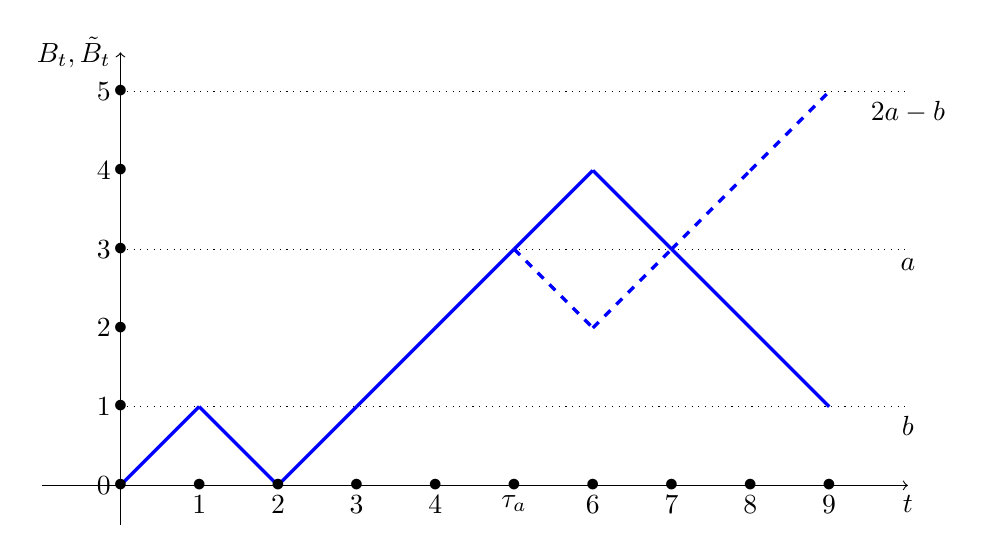
\begin{tikzpicture}[scale=1]
  %Origin and axis
  \coordinate (O) at (0,0);
  \draw[->] (-1,0) -- (10,0) coordinate[label = {below:$t$}] (xmax);
  \draw[-, dotted] (0,1) -- (10,1) coordinate[label = {below:$b$}] (b);
  \draw[-, dotted] (0,3) -- (10,3) coordinate[label = {below:$a$}] (a);
  \draw[-, dotted] (0,5) -- (10,5) coordinate[label = {below:$2a-b$}] (2a-b);
  \draw[->] (0,-0.5) -- (0,5.5) coordinate[label = {left:$B_t, \tilde{B}_t$}] (ymax);
  %Lower linear boundary


  %Stochastic process trajectory

  \draw (0,0) node[blue,left] {} node{};
  \draw[very thick,blue,-] (0,0) -- (1,1) node[pos=0.5, above] {} ;
  \draw[very thick,blue] (1,1) -- (2,0) node[pos=0.5, right] {};
  \draw[very thick,blue] (2,0) -- (3,1) node[pos=0.5, right] {};
  \draw[very thick,blue] (3,1) -- (4,2) node[pos=0.5, right] {};
  \draw[very thick,blue] (4,2) -- (5,3) node[pos=0.5, right] {};
  
  %reflected
  \draw[very thick,dashed,blue] (5,3) -- (6,2) node[pos=0.5, right] {};
  \draw[very thick,dashed,blue] (6,2) -- (7,3) node[pos=0.5, right] {};
  \draw[very thick,dashed, blue] (7,3) -- (8,4) node[pos=0.5, right] {};
  \draw[very thick,dashed, blue] (8,4) -- (9,5) node[pos=0.5, right] {};

  % Not reflected
  \draw[very thick,blue] (5,3) -- (6,4) node[pos=0.5, right] {};
  \draw[very thick,blue] (6,4) -- (7,3) node[pos=0.5, right] {};
  \draw[very thick,blue] (7,3) -- (8,2) node[pos=0.5, right] {};
  \draw[very thick,blue] (8,2) -- (9,1) node[pos=0.5, right] {};
  
  %Jump Times
  \draw (1,0) node[below] {$1$} node{ $\bullet$};
  \draw (2,0) node[below] {$2$} node{ $\bullet$};
  \draw (3,0) node[below] {$3$} node{ $\bullet$};
  \draw (4,0) node[below] {$4$} node{ $\bullet$};
  \draw (5,0) node[below] {$\tau_a$} node{ $\bullet$};
  \draw (6,0) node[below] {$6$} node{ $\bullet$};
  \draw (7,0) node[below] {$7$} node{ $\bullet$};
  \draw (8,0) node[below] {$8$} node{ $\bullet$};
  \draw (9,0) node[below] {$9$} node{ $\bullet$};
  %Level of the counting process
   \draw (0,0) node[black,left] {$0$} node{ \color{black}$\bullet$};
   \draw (0,1) node[black,left] {$1 $} node{ \color{black}$\bullet$};
   \draw (0,2) node[black,left] {$2$} node{ \color{black}$\bullet$};
   \draw (0,3) node[black,left] {$3$} node{ \color{black}$\bullet$};
   \draw (0,4) node[black,left] {$4$} node{ \color{black}$\bullet$};
   \draw (0,5) node[black,left] {$5 $} node{ \color{black}$\bullet$};
\end{tikzpicture}
\end{center}
\caption{Une trajectoire du mouvement brownien $(B_t)_{t\geq 0}$ et de son processus réfléchi $(\tilde{B}_t)_{t\geq0}$.}
\label{fig:trajectory_reflected_bm}
\end{figure}
La \cref{fig:trajectory_reflected_bm} montre la bijection entre les trajectoires de $B_t$ qui vont du niveau $a$ au niveau $b$ et celles qui vont de $a$ à $2a - b$ entre $\tau_a$ et $t$. Le processus réfléchi à partir de $\tau_a$ se comporte comme un mouvement brownien issu de $a$ après $\tau_a$. On a 
\begin{eqnarray*}
\Prob(\tau_a\leq t, B_t \leq  b)&=&\Prob(\tau_a\leq t, \tilde{B}_t \geq  2a-b)\\
&=&\Prob(\tau_a\leq t, B_t \geq  2a-b)\\
&=&\Prob( B_t \geq  2a-b).
\end{eqnarray*}
Pour la second assertion, on note que 
\begin{eqnarray*}
\Prob(S_t \geq a ) &=&\Prob(S_t \geq a, B_t \leq a ) + \Prob(S_t \geq a, B_t > a )\\
&=&\Prob(S_t \geq a, B_t \leq a ) + \Prob( B_t > a )\\
&=&\Prob( B_t > a ) +  \Prob( B_t > a )\\
&=&2\Prob( B_t > a )\\
&=&\Prob( -B_t < a ) + \Prob( B_t > a )\\
&=&\Prob( |B_t| > a ).
\end{eqnarray*}
\end{proof}

\section{Variante du mouvement Brownien et application}
\subsection{Le mouvement brownien avec dérive}
\begin{definition}
Soit $(B_t)_{t\geq 0}$ un mouvement brownien. Pour $\mu\in \RL$ et $\sigma>0$, le processus 
$$
X_t = \mu t+\sigma B_t,\text{ }t\geq0,
$$
est le mouvement brownien avec dérive de paramètre de tendance $\mu$ et de variance (ou volatilité) $\sigma$.
\end{definition}
\begin{ex}
Le processus 
$$
X_t = x+ct +\sigma B_t-\sum_{i=1}^{N_t}U_i,\text{ }t\geq 0,
$$
est le processus de ruine perturbé par le mouvement brownien. l'ajout du mouvement brownien permet d'ajouter des fluctuations dans le processus de collecte des primes par exemple. 
\end{ex}
\subsection{Le mouvement brownien géométrique}
\begin{definition}
Soit $(X_t)_{t\geq 0}$ un mouvement brownien avec dérive de paramètre $\mu$ et $\sigma$. Le processus 
$$
S_t = S_0\e^{X_t},\text{ }t\geq0,
$$
est le mouvement brownien géométrique.
\end{definition}
Le mouvement brownien géométrique est utilisé pour modéliser le prix des actifs financier. Il est toujours positif et conduit à des rendements $S_t/S_{t-1}$ \iid de loi lognormal, ce qui signifie que les log rendements vérifient 
$$
\log \left(\frac {S_t }{S_{t-1}}\right)\sim\NormalDist(\mu, \sigma).
$$ 
\subsection{Le pont brownien}
\begin{definition}
Soit $(B_t)_{t\geq 0}$ un mouvement brownien. Le processus 
$$
X_t = B_t| B_1 = 0\text{ pour }0\leq t\leq 1,
$$
est un pont brownien. 
\end{definition}
Le pont brownien est un processus gaussien. En effet, 
$$
B_t|B_1 = 0\sim \NormalDist\left(0, t(1-t)\right)
$$
La fonction de moyenne est donnée par
$$
m(t) = 0.
$$
La fonction de covariance, pour $s< t$ est donnée par 
\begin{eqnarray*}
C(s,t)&=&\Cov(X_s, X_t)\\
&=&\E(X_s X_t)\\
&=&\E(B_s B_t|B_1 = 0)\\
&=&\E(\E(B_s B_t|B_t)|B_1 = 0)\\
&=&\E(B_t\E(B_s |B_t)|B_1 = 0)\\
&=&\E\left(B_t\frac{s}{t}B_t|B_1 = 0\right)\\
&=&\frac{s}{t}\E\left(B_t^2|B_1 = 0\right)\\
&=&\frac{s}{t}t(1-t)\\
&=&s-st\\
\end{eqnarray*}
par symétrie $C(s,t) = t-st$ si $t<s$. On en déduit que 
$$
C(s,t) = s\land t - st
$$
\begin{prop}
Le processus défini par 
$$
X_t = B_t - tB_1,\text{ }0\leq t\leq 1,
$$
est un pont brownien.
\end{prop}
\begin{proof}
On montre que $X_t$ est un processus gaussien dont la fonction de moyenne et de covariance est la même que celle du pont brownien. 
\end{proof}
\begin{ex}
Le pont brownien apparait dans le test d'adéquation à la loi uniforme de Kolmogorv-Smirnov. Supposons que nous soyons en présence d'un échantillon $U_1,\ldots, U_n$ d'observation comprise entre $0$ et $1$. Nous souhaitons tester l'adéquation de la loi $\UnifDist([0,1])$. Nous comparons donc la fonction de répartition empirique 
$$
F_n(t) = \sum_{i=1}^n\ind_{U_i\leq t}
$$
avec la fonction de répartition de la loi uniforme donnée par 
$$
F(t) = t\text{ pour }0\leq t\leq 1.
$$
Le test de Kolmogorov-Smirnov considère la distance 
$$
D_n = \sup_{0\leq t\leq 1}|F_n(t)-t|
$$
Soit le processus $X_t = \sqrt{n}[F_n(t)-t],\text{ }0\leq t\leq 1$. Sous $H_0$ les données proviennent de la loi uniforme et donc d'après le théorème centrale limite 
$$
X_t\sim\NormalDist(0, t(1-t)),\text{ pour }n\rightarrow \infty.
$$
de plus $X_0 = 0$ et $X_1 = 0$. On peut montrer que le $X_t$ converge effectivement vers un pont brownien en utilisant le principe d'invariance de Donsker. Le test repose alors sur la loi de $\sup_{0\leq t\leq 1} X_t$, le maximum atteint par le pont brownien.
\end{ex}
